% Discription of what ROS is and what it does

\chapter{Robot Operating System\authorA}

\section{What is the Robot Operating System?}
The Robot Operating System, which is also known as ROS, is a flexible framework for writing software that gets utilized on robots. It was founded by Willow Garage in 2012 and gets primarily maintained by the Open Source Robotics Foundation (OSRF) \cite{osrf}. In Europe the project gets coordinated by the Fraunhofer IPA in form of the \textit{ROS Industrial Consortium Europe}. ROS is a middle-ware which is not a operating system but provides services that manage hardware abstraction, low-level device control, message-passing between processes and package management. \emph{\glqq It is a collection of tools, libraries, and conventions that aim to simplify the task of creating complex and robust robot behavior across a wide variety of robotic platforms.\grqq}~\cite{aboutros}

\section{Design}
The processes of ROS are represented in nodes which are in a graph structure. Everything gets managed by a single process called \textit{ROS Master}, to whom all other nodes register on startup. But instead of sending all of the messages over the master, the master sets up a peer-to-peer connection between the nodes. This decentralized architecture is helpful as many robots consists of many computer hardware which is connected via a network and are likely to transfer big messages. \cite{rosoneoone}   \\
\begin{figure}[h]
	\centering
	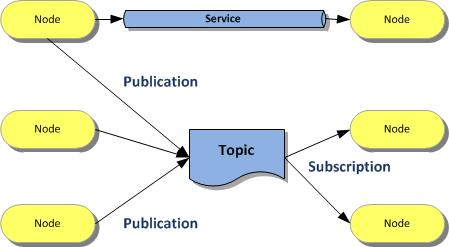
\includegraphics[width=0.7\textwidth]{./media/images/ros_structure.jpg}
  	\caption{ROS structure
  	\\Source: https://tinyurl.com/yyfthk7c}
  	\label{rosstructure}
\end{figure}

\subsection{Topics}
It is based on a topic system, where a topic acts like a bus over which nodes send and receive messages. Each topic must be unique in it's name, which is usually set by the developer. The process of publishing and subscribing is handles anonymously so that no node knows which nodes are sending and receiving messages on a certain topic.

\subsection{Nodes}
A node, which represent a single running process, can provide data using a matching topic and publish it to the system, where theoretically every other node can subscribe to it, to get the data. 

\section{Licenses and OS}
The language-independent tools and the main client libraries have men released under the BSD license and as such they are open source software for commercial and research use. The majority of 3rd party packages are released under several other open-source licenses.\newline
The ROS libraries are geared toward a UNIX-System which is mainly due to their dependence on a large collection of open source software and libraries.
For example \textit{Ubuntu} is in the list of supported operating systems, while others like \textit{Fedora, MacOS and Windows} are "experimental" and are mainly supported by the community.

\section{Tools}
One of the core functionalities that ROS provides are the tools which allow the developers to visualize 2D and 3D data, record data, easily navigating ROS packages, creating complex scripts that configure and setup processes. Thanks to this tools it simplifies and provides solution for common robotic development.

\subsection{Rosbag}
Rosbag is a tool that can be used over the command line to record, playback and store ROS message data. The data gets stored in a file called bag, where it records the messages as they come in. It's possible to play these bag files. By doing this the recorded messages get published into the system, as they where live. It's very handy if you need data for later development or to use a bunch of different scenarios for testing

\subsection{RQt}
RQt provides a graphical overview of the ROS computation graph. It shows the nodes and how they are connected to each other. It also shows if a node is even subscribing to a topic or publishes something. Other than that it can be used to subscribe to different topics and show them directly in RQt.
\begin{figure}[h]
	\centering
	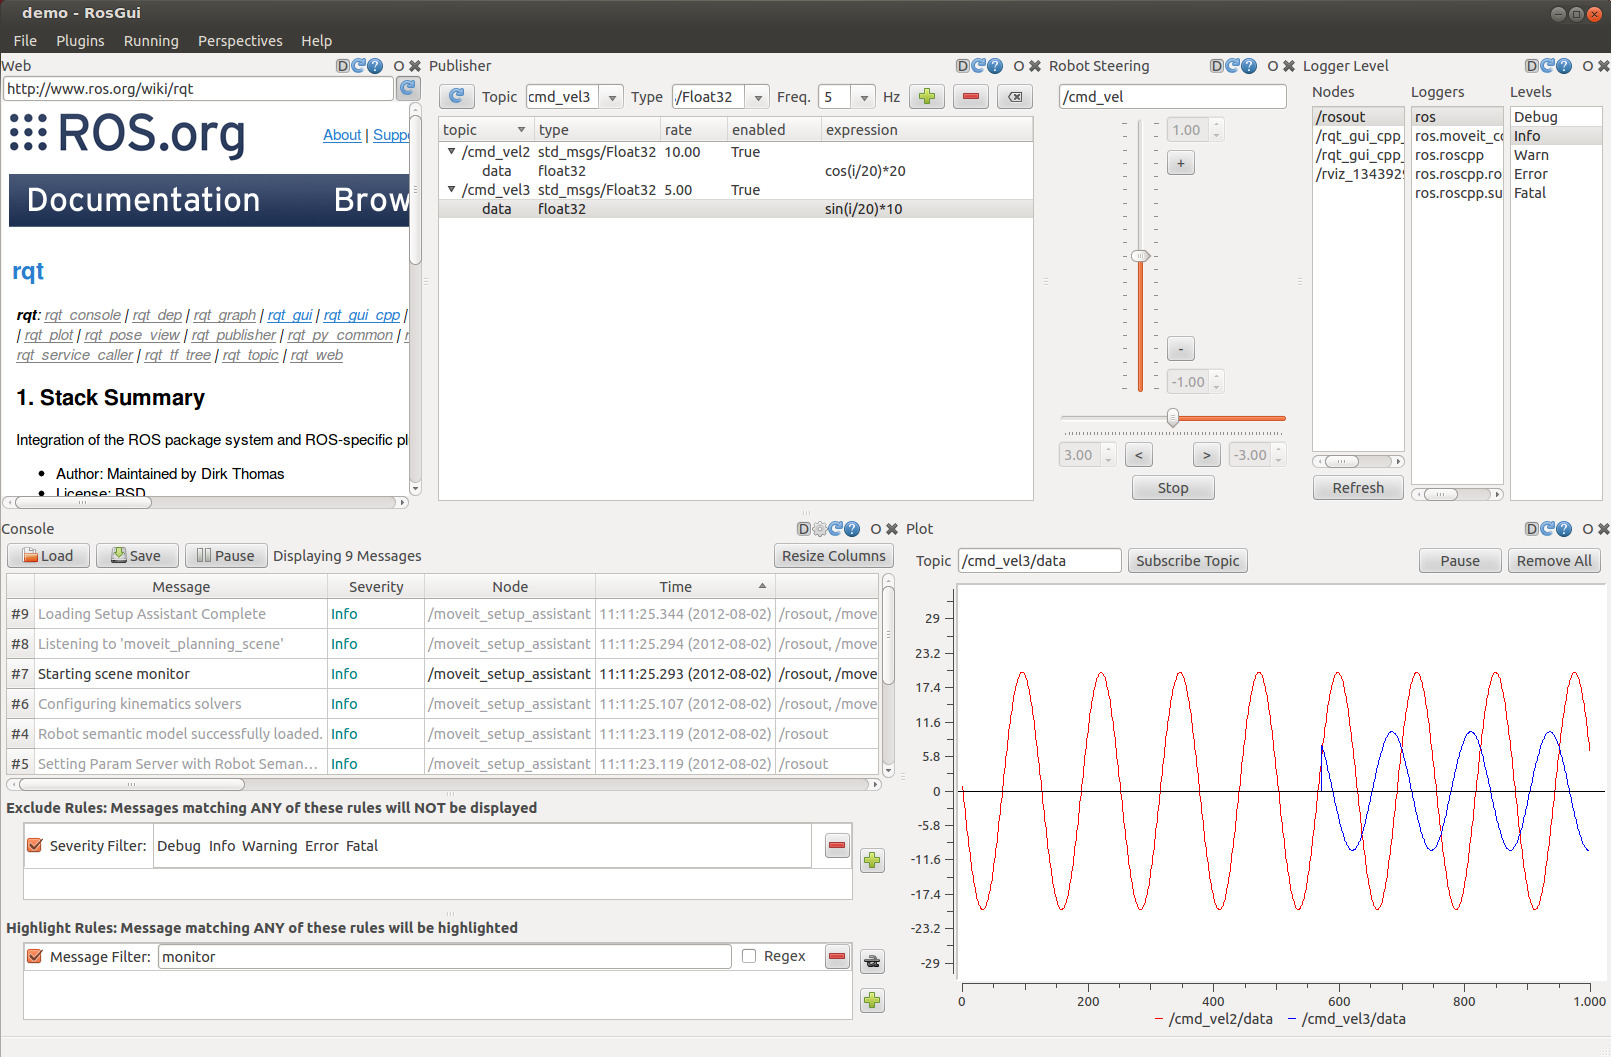
\includegraphics[width=0.6\textwidth]{./media/images/RQt}
  	\caption{RQt interface\\Source: https://wiki.ros.org/RQt}
  	\label{rqtinterface}
\end{figure}

\subsection{CatKin}
Catkin is the newer ROS build system, which compiles the files in the source folder. It is based on CMake and is cross-platform and language-independent as most other ROS tools.

\subsection{Rviz}
A visualizer for three-dimensional data where robots, environments and sensor information can be visualized. It is highly customise able with display many types of visualisation and plugin support. \\
\begin{figure}[h]
	\centering
	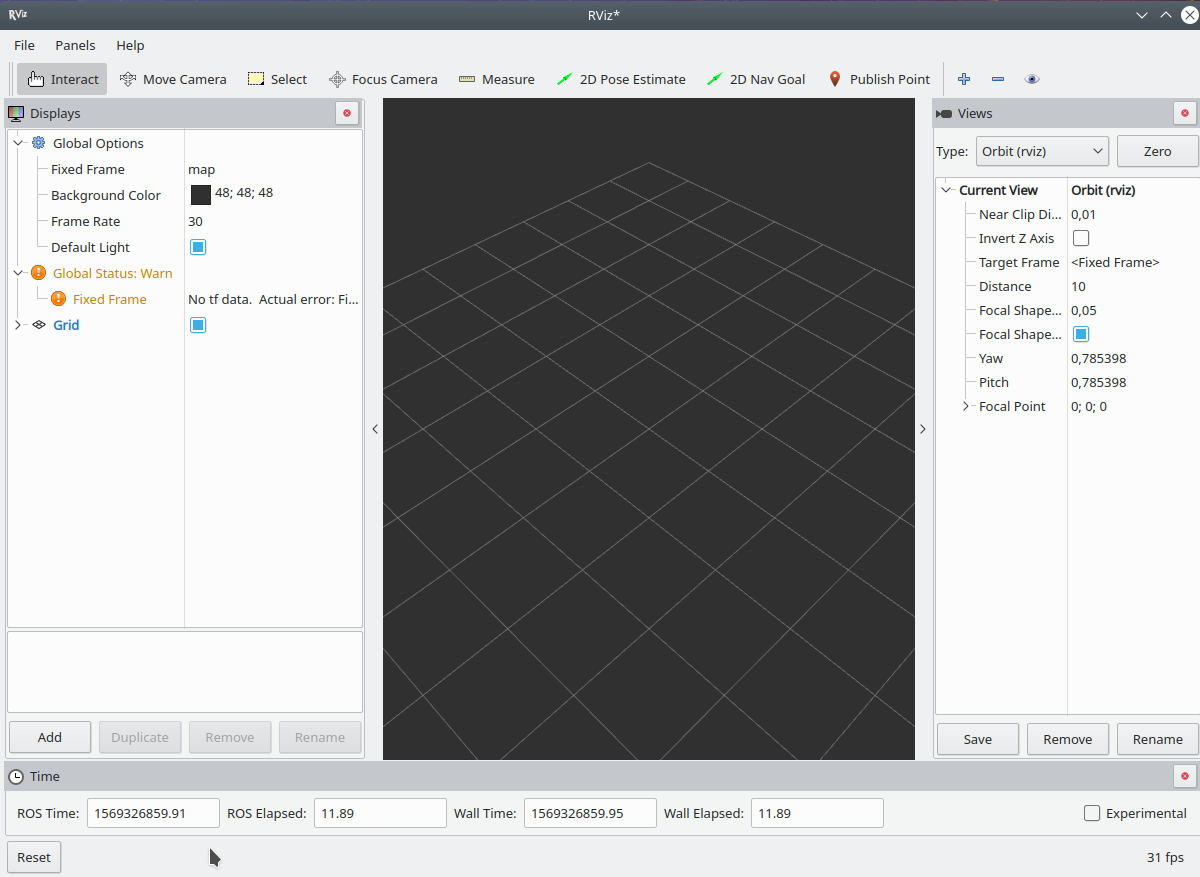
\includegraphics[width=0.7\textwidth]{./media/images/rviz}
  	\caption{Rviz interface}
  	\label{rvizinterface}
\end{figure}

\subsection{Roslaunch}
Roslaunch is a tool for launching multiple ROS nodes and setting parameters on startup. It can be used to launch nodes locally or remotely on a server.
The configuration for a start script is written in a launch file using XML. In these files it's easy to make a automated startup and configuration process to be executed with one command. It's possible to execute launch files in other launch files to chain them together.